\documentclass[a4paper,openwrite,12pt]{article}
\usepackage[utf8]{inputenc}
\usepackage{graphicx}
\usepackage{titling}
\usepackage[spanish]{babel}
\usepackage{float}
\usepackage{amsmath}
\usepackage{booktabs}
\usepackage{listings}


\begin{document}

\begin{titlepage}

\begin{center}
\vspace*{-1in}
\begin{figure}[htb]
\begin{center}

\includegraphics[width=8cm]{img/udc.png}
\end{center}
\end{figure}

\vspace*{1in}
ICBio 20/21 \\
\vspace*{1in}
\begin{Large}
\textbf{P3\&P4} \\
\end{Large}

\vspace*{3in}

\begin{large}
\raggedleft
\textbf{Autores:}Sergio Rodríguez Nieto \\
David Maseda Neira \\
\textbf{Fecha:}\textit{Coruña,a \today}\\
\end{large}

\end{center}
\end{titlepage} 
\pagenumbering{gobble}
\tableofcontents
\pagenumbering{arabic}
\newpage
\section{Introducción}
En esta memoria incremental se presentan el procedimiento y los resultados de las prácticas en Inteligencia Computacional para la Bioinformática.

\section{Descripción de los \textit{datasets}}
\subsection{\textit{Breast Cancer Wisconsin Dataset}}
Consiste en  683 ejemplos, con 10 características por ejemplo:
\begin{itemize}
    \item Radio
    \item Textura
    \item Perímetro
    \item Área
    \item Suavidad
    \item Compacidad
    \item Concavidad
    \item Puntos de concavidad
    \item Simetría
    \item Dimensión fractal
\end{itemize}

Los ejemplos se clasifican como malignos(1) o benignos(2).

\subsection{\textit{Iris Flower Dataset}}
Consiste en 150 ejemplos, 50 para cada una de las 3 clases (Setosa, Versicolor y Virginica)
Contiene 4 características por ejemplo:
\begin{itemize}
    \item Longitud del sépalo (cm)
    \item Anchura del sépalo (cm)
    \item Longitud del pétalo (cm)
    \item Anchura del pétalo (cm)
\end{itemize}

\section{Preparación del \textit{dataset}}
\subsection{Preparación del \textit{Breast Cancer Wisconsin Dataset}}
Los datos del \textit{Breast Cancer Wisconsin Dataset} se obtienen en un CSV.
Durante esta práctica, no se realiza extracción de características, por lo que la carga de los datos del CSV se realiza directamente. Estos datos se guardan en un fichero MAT de matlab, para no volver a parsear el csv en posteriores ejecuciones. De igual modo, de realizarse preprocesado, este solo sería necesario la primera vez, al construir el dataset.

\subsection{Preparación del \textit{Iris Flower Dataset}}
De igual manera que con el \textit{dataset} anterior, no se realiza preprocesado, y los datos se guardan en un fichero de matlab para posterior acceso.

\subsection{\textit{Biodeg Dataset}}
El dataset contiene 1055 instancias de sustancias químicas.
Cada una de ellas consiste en 41 descriptores moleculares, usados para clasificar en 2 clases: Ready Biodegradable(RB) y Not Ready Biodegradable(NRB).

\subsection{Henon Map}
El dataset de Henon es una serie temporal caótica, que mapea un punto $(x_n,y_n) => (x_{n+1},y_{n+1})$.
Para este trabajo, se utilizarán 1500 muestras, agrupadas en ventanas deslizantes de 10 y 20 elementos.

\section{Metodología y desarrollo}

El código está organizado de la siguiente manera:

Existen 8 módulos:

\begin{itemize}
    \item lineal.m
    \item quadratic.m
    \item Tree.m
    \item SVM.m
    \item SVM\_Multiclass.m
    \item SVM\_Regressor.m
    \item ANN.m
    \item ANN\_Regressor.m
\end{itemize}



El parámetro debug en \textit{Tree.m} sirve para ocultar las figuras de la estructura de los árboles, por simplicidad al ejecutar. Si se quiere consultar la estructura de los árboles, se fija el parámetro debug a true.

Para cada uno de los modelos, la función que define ejecuta secuencialmente lo siguiente:

\begin{enumerate}
    \item Carga los datos del dataset provisto en la firma de la función.
    \item Configura los parámetros para el modelo según lo definido en la firma de la función.
    \item Entrena el modelo y lo valida con el \textit{split} de test.
    \item Muestra las métricas por clase y globales.
    \item La función devuelve el accuracy, tanto en train como en test.
\end{enumerate}

\subsection{Ejecución}
Se provee un archivo main.m, que construye y ejecuta todos los modelos para ambos \textit{datasets}. 
\textbf{IMPORTANTE}: Se ha utilizado el bloque \textbf{arguments} de MATLAB, que sólamente está disponible de la versión 2019b en adelante, por lo cual si se ejecuta en una versión anterior, muestra un error de sintaxis.
\section{Modelos y entrenamiento} 
Se prueban 5 modelos diferentes:
Un discriminante lineal, un discriminante cuadrático y 3 variaciones de árboles de clasificación, con variaciones en los parámetros.
Todos los modelos se entrenan con un \textit{10-fold}.
Se recogen las siguientes métricas de rendimiento:
\begin{itemize}
    \item Recall
    \item Precisión
    \item Especificidad
    \item VPN
    \item Accuracy
    \item F1
\end{itemize}

En esta sección, se presentan los modelos, sus parámetros, y los resultados para el conjunto de test.

\subsection{Discriminante lineal}

\begin{table}[H]
\centering
\begin{tabular}{@{}lllll@{}}
\toprule
            & Setosa & Versicolor & Virginica &  \\ \midrule
Recall      & 1.00   & 0.96       & 0.98      &  \\
Precision   & 1.00   & 0.98       & 0.96      &  \\
Specificity & 1.00   & 0.96       & 0.98      &  \\
VPN         & 1.00   & 0.98       & 0.99      &  \\
Accuracy    & 1.00   & 0.98       & 0.98      &  \\
F1          & 1.00   & 0.97       & 0.97      &  \\ \bottomrule
\end{tabular}
\caption{Iris(lineal)}
\end{table}


\begin{table}[H]
\centering
\begin{tabular}{@{}llll@{}}
\toprule
            & Maligno & Benigno &  \\ \midrule
Recall      & 0.98    & 0.92    &  \\
Precision   & 0.96    & 0.97    &  \\
Specificity & 0.98    & 0.92    &  \\
VPN         & 0.97    & 0.97    &  \\
Accuracy    & 0.96    & 0.96    &  \\
F1          & 0.97    & 0.94    &  \\ \bottomrule
\end{tabular}
\caption{Cáncer(lineal)}
\end{table}


\begin{table}[H]
\centering
\begin{tabular}{@{}llll@{}}
\toprule
            & NRB &   RB &  \\ \midrule
Recall      & 0.91    & 0.77    &  \\
Precision   & 0.89    & 0.81    &  \\
Specificity & 0.91    & 0.77    &  \\
VPN         & 0.81    & 0.89    &  \\
Accuracy    & 0.86    & 0.86    &  \\
F1          & 0.89    & 0.78    &  \\ \bottomrule
\end{tabular}
\caption{Biodeg(lineal)}
\end{table}



\subsection{Discriminante cuadrático}


\begin{table}[H]
\centering
\begin{tabular}{@{}lllll@{}}
\toprule
            & Setosa & Versicolor & Virginica &  \\ \midrule
Recall      & 1.00   & 0.92       & 0.98      &  \\
Precision   & 1.00   & 0.98       & 0.94      &  \\
Specificity & 1.00   & 0.92       & 0.98      &  \\
VPN         & 1.00   & 0.97       & 0.99      &  \\
Accuracy    & 1.00   & 0.97       & 0.97      &  \\
F1          & 1.00   & 0.94       & 0.96      &  \\ \bottomrule
\end{tabular}
\caption{Iris(Quad)}
\end{table}


\begin{table}[H]
\centering
\begin{tabular}{@{}llll@{}}
\toprule
            & Maligno & Benigno &  \\ \midrule
Recall      & 0.94    & 0.98    &  \\
Precision   & 0.99   & 0.90    &  \\
Specificity & 0.94    & 0.98    &  \\
VPN         & 0.90    & 0.99    &  \\
Accuracy    & 0.95    & 0.95    &  \\
F1          & 0.96    & 0.94    &  \\ \bottomrule
\end{tabular}
\caption{Cáncer(Quad)}
\end{table}

Nota: El predictor en el discriminante cuadrático para el dataset de Biodeg no encuentra varianza para la clase RB. Se utiliza en su lugar el discriminante ´pseudoQuadratic´
\begin{table}[H]
\centering
\begin{tabular}{@{}llll@{}}
\toprule
            & NRB &   RB &  \\ \midrule
Recall      & 0.75    & 0.90    &  \\
Precision   & 0.93    & 0.65    &  \\
Specificity & 0.76    & 0.90    &  \\
VPN         & 0.65    & 0.93    &  \\
Accuracy    & 0.80    & 0.80    &  \\
F1          & 0.83    & 0.75    &  \\ \bottomrule
\end{tabular}
\caption{Biodeg(quad)}
\end{table}


\subsection{Árbol 1}

Árbol de búsqueda con los parámetros por defecto:

\begin{itemize}
    \item MinLeafSize: 1
    \item MinParentSize: 10
\end{itemize}

\begin{table}[H]
\centering
\begin{tabular}{@{}lllll@{}}
\toprule
            & Setosa & Versicolor & Virginica &  \\ \midrule
Recall      & 1.00   & 0.90       & 0.92      &  \\
Precision   & 1.00   & 0.93       & 0.91      &  \\
Specificity & 1.00   & 0.90       & 0.92      &  \\
VPN         & 1.00   & 0.95       & 0.96      &  \\
Accuracy    & 1.00   & 0.94       & 0.94      &  \\
F1          & 1.00   & 0.91       & 0.91      &  \\ \bottomrule
\end{tabular}
\caption{Iris(Tree 1)}
\end{table}


\begin{table}[H]
\centering
\begin{tabular}{@{}llll@{}}
\toprule
            & Maligno & Benigno &  \\ \midrule
Recall      & 0.96    & 0.91    &  \\
Precision   & 0.95    & 0.92    &  \\
Specificity & 0.96    & 0.91    &  \\
VPN         & 0.92    & 0.95    &  \\
Accuracy    & 0.94    & 0.94    &  \\
F1          & 0.95    & 0.91    &  \\ \bottomrule
\end{tabular}
\caption{Cáncer(Tree 1)}
\end{table}


\begin{table}[H]
\centering
\begin{tabular}{@{}llll@{}}
\toprule
            & NRB &   RB &  \\ \midrule
Recall      & 0.87    & 0.71    &  \\
Precision   & 0.86    & 0.73    &  \\
Specificity & 0.87    & 0.71    &  \\
VPN         & 0.73    & 0.86    &  \\
Accuracy    & 0.82    & 0.82    &  \\
F1          & 0.86    & 0.72    &  \\ \bottomrule
\end{tabular}
\caption{Biodeg(Tree 1)}
\end{table}


\subsection{Árbol 2}
Árbol de búsqueda con los parámetros:

\begin{itemize}
    \item MinLeafSize: 5
    \item MinParentSize: 10
\end{itemize}

\begin{table}[H]
\centering
\begin{tabular}{@{}lllll@{}}
\toprule
            & Setosa & Versicolor & Virginica &  \\ \midrule
Recall      & 1.00   & 0.94       & 0.88      &  \\
Precision   & 1.00   & 0.90       & 0.94      &  \\
Specificity & 1.00   & 0.95       & 0.89      &  \\
VPN         & 1.00   & 0.97       & 0.95      &  \\
Accuracy    & 1.00   & 0.94       & 0.94      &  \\
F1          & 1.00   & 0.92       & 0.90      &  \\ \bottomrule
\end{tabular}
\caption{Iris(Tree 2)}
\end{table}


\begin{table}[H]
\centering
\begin{tabular}{@{}llll@{}}
\toprule
            & Maligno & Benigno &  \\ \midrule
Recall      & 0.96    & 0.92    &  \\
Precision   & 0.96    & 0.93    &  \\
Specificity & 0.96    & 0.92    &  \\
VPN         & 0.93    & 0.96    &  \\
Accuracy    & 0.95    & 0.95    &  \\
F1          & 0.96    & 0.92    &  \\ \bottomrule
\end{tabular}
\caption{Cáncer(Tree 2)}
\end{table}

\begin{table}[H]
\centering
\begin{tabular}{@{}llll@{}}
\toprule
            & NRB &   RB &  \\ \midrule
Recall      & 0.87    & 0.67    &  \\
Precision   & 0.84    & 0.72    &  \\
Specificity & 0.87    & 0.67    &  \\
VPN         & 0.72    & 0.84    &  \\
Accuracy    & 0.80    & 0.80    &  \\
F1          & 0.85    & 0.69    &  \\ \bottomrule
\end{tabular}
\caption{Biodeg(Tree 2)}
\end{table}


\subsection{Árbol 3}
Árbol de búsqueda con los parámetros:

\begin{itemize}
    \item MinLeafSize: 2
    \item MinParentSize: 5
\end{itemize}

\begin{table}[H]
\centering
\begin{tabular}{@{}lllll@{}}
\toprule
            & Setosa & Versicolor & Virginica &  \\ \midrule
Recall      & 1.00   & 0.94       & 0.90      &  \\
Precision   & 1.00   & 0.92       & 0.94      &  \\
Specificity & 1.00   & 0.94       & 0.90      &  \\
VPN         & 1.00   & 0.97       & 0.95      &  \\
Accuracy    & 1.00   & 0.95       & 0.95      &  \\
F1          & 1.00   & 0.92       & 0.92      &  \\ \bottomrule
\end{tabular}
\caption{Iris(Tree 3)}
\end{table}


\begin{table}[H]
\centering
\begin{tabular}{@{}llll@{}}
\toprule
            & Maligno & Benigno &  \\ \midrule
Recall      & 0.97    & 0.92    &  \\
Precision   & 0.96    & 0.95    &  \\
Specificity & 0.97    & 0.92    &  \\
VPN         & 0.95    & 0.96    &  \\
Accuracy    & 0.95    & 0.95    &  \\
F1          & 0.97    & 0.93    &  \\ \bottomrule
\end{tabular}
\caption{Cáncer(Tree 3)}
\end{table}

\begin{table}[H]
\centering
\begin{tabular}{@{}llll@{}}
\toprule
            & NRB &   RB &  \\ \midrule
Recall      & 0.85    & 0.73    &  \\
Precision   & 0.86    & 0.71    &  \\
Specificity & 0.85    & 0.73    &  \\
VPN         & 0.71    & 0.86    &  \\
Accuracy    & 0.81    & 0.81    &  \\
F1          & 0.85    & 0.72    &  \\ \bottomrule
\end{tabular}
\caption{Biodeg(Tree 3)}
\end{table}

\subsection{SVM 1}
SVM con los parámetros:
\begin{itemize}
    \item KernelFunction: polynomial
    \item onevsone
\end{itemize}

\begin{table}[H]
\centering
\begin{tabular}{@{}lllll@{}}
\toprule
            & Setosa & Versicolor & Virginica &  \\ \midrule
Recall      & 1.00   & 0.98       & 0.98      &  \\
Precision   & 1.00   & 0.98       & 0.98      &  \\
Specificity & 1.00   & 0.98       & 0.98      &  \\
VPN         & 1.00   & 0.99       & 0.99      &  \\
Accuracy    & 1.00   & 0.99       & 0.99      &  \\
F1          & 1.00   & 0.98       & 0.98      &  \\ \bottomrule
\end{tabular}
\caption{Iris(SVM 1)}
\end{table}


\begin{table}[H]
\centering
\begin{tabular}{@{}llll@{}}
\toprule
            & Maligno & Benigno &  \\ \midrule
Recall      & 0.97    & 0.90    &  \\
Precision   & 0.95    & 0.94    &  \\
Specificity & 0.97    & 0.90    &  \\
VPN         & 0.94    & 0.95    &  \\
Accuracy    & 0.95    & 0.95    &  \\
F1          & 0.96    & 0.92    &  \\ \bottomrule
\end{tabular}
\caption{Cáncer(SVM 1)}
\end{table}


\begin{table}[H]
\centering
\begin{tabular}{@{}llll@{}}
\toprule
            & NRB &   RB &  \\ \midrule
Recall      & 0.86    & 0.80    &  \\
Precision   & 0.89    & 0.74    &  \\
Specificity & 0.86    & 0.80    &  \\
VPN         & 0.74    & 0.89    &  \\
Accuracy    & 0.84    & 0.84    &  \\
F1          & 0.87    & 0.76    &  \\ \bottomrule
\end{tabular}
\caption{Biodeg(SVM 1)}
\end{table}

\subsection{SVM 2}
SVM con los parámetros:
\begin{itemize}
    \item KernelFunction: polynomial
    \item PolynomialOrder: 5
    \item onevsall
\end{itemize}

\begin{table}[H]
\centering
\begin{tabular}{@{}lllll@{}}
\toprule
            & Setosa & Versicolor & Virginica &  \\ \midrule
Recall      & 1.00   & 1.00       & 1.00      &  \\
Precision   & 1.00   & 1.00       & 1.00      &  \\
Specificity & 1.00   & 1.00       & 1.00      &  \\
VPN         & 1.00   & 1.00       & 1.00      &  \\
Accuracy    & 1.00   & 1.00       & 1.00      &  \\
F1          & 1.00   & 1.00       & 1.00      &  \\ \bottomrule
\end{tabular}
\caption{Iris(SVM 2)}
\end{table}


\begin{table}[H]
\centering
\begin{tabular}{@{}llll@{}}
\toprule
            & Maligno & Benigno &  \\ \midrule
Recall      & 0.97    & 0.87    &  \\
Precision   & 0.93    & 0.93    &  \\
Specificity & 0.97    & 0.87    &  \\
VPN         & 0.93    & 0.93    &  \\
Accuracy    & 0.93    & 0.93    &  \\
F1          & 0.95    & 0.90    &  \\ \bottomrule
\end{tabular}
\caption{Cáncer(SVM 2)}
\end{table}


\begin{table}[H]
\centering
\begin{tabular}{@{}llll@{}}
\toprule
            & NRB &   RB &  \\ \midrule
Recall      & 0.94    & 0.10    &  \\
Precision   & 0.67    & 0.45    &  \\
Specificity & 0.94    & 0.10    &  \\
VPN         & 0.45    & 0.67    &  \\
Accuracy    & 0.65    & 0.65    &  \\
F1          & 0.78    & 0.00    &  \\ \bottomrule
\end{tabular}
\caption{Biodeg(SVM 2)}
\end{table}

\subsection{SVM 3}
SVM con los parámetros:
\begin{itemize}
    \item KernelFunction: polynomial
    \item PolynomialOrder: 6
\end{itemize}

\begin{table}[H]
\centering
\begin{tabular}{@{}lllll@{}}
\toprule
            & Setosa & Versicolor & Virginica &  \\ \midrule
Recall      & 1.00   & 1.00       & 1.00      &  \\
Precision   & 1.00   & 1.00       & 1.00      &  \\
Specificity & 1.00   & 1.00       & 1.00      &  \\
VPN         & 1.00   & 1.00       & 1.00      &  \\
Accuracy    & 1.00   & 1.00       & 1.00      &  \\
F1          & 1.00   & 1.00       & 1.00      &  \\ \bottomrule
\end{tabular}
\caption{Iris(SVM 3)}
\end{table}


\begin{table}[H]
\centering
\begin{tabular}{@{}llll@{}}
\toprule
            & Maligno & Benigno &  \\ \midrule
Recall      & 0.95    & 0.93    &  \\
Precision   & 0.98    & 0.92    &  \\
Specificity & 0.98    & 0.93    &  \\
VPN         & 0.99    & 0.96    &  \\
Accuracy    & 0.98    & 0.95    &  \\
F1          & 0.96    & 0.93    &  \\ \bottomrule
\end{tabular}
\caption{Cáncer(SVM 3)}
\end{table}

\begin{table}[H]
\centering
\begin{tabular}{@{}llll@{}}
\toprule
            & NRB &   RB &  \\ \midrule
Recall      & 0.69    & 0.33    &  \\
Precision   & 0.71    & 0.33    &  \\
Specificity & 0.69    & 0.33    &  \\
VPN         & 0.33    & 0.71    &  \\
Accuracy    & 0.57    & 0.57    &  \\
F1          & 0.61    & 0.00    &  \\ \bottomrule
\end{tabular}
\caption{Biodeg(SVM 3)}
\end{table}


\subsection{SVM 4}
SVM con los parámetros:
\begin{itemize}
    \item KernelFunction: rbf
    \item onevsall
\end{itemize}

\begin{table}[H]
\centering
\begin{tabular}{@{}lllll@{}}
\toprule
            & Setosa & Versicolor & Virginica &  \\ \midrule
Recall      & 1.00   & 0.98       & 0.98      &  \\
Precision   & 1.00   & 0.98       & 0.98      &  \\
Specificity & 1.00   & 0.98       & 0.98      &  \\
VPN         & 1.00   & 0.99       & 0.99      &  \\
Accuracy    & 1.00   & 0.99       & 0.99      &  \\
F1          & 1.00   & 0.98       & 0.98      &  \\ \bottomrule
\end{tabular}
\caption{Iris(SVM 4)}
\end{table}


\begin{table}[H]
\centering
\begin{tabular}{@{}llll@{}}
\toprule
            & Maligno & Benigno &  \\ \midrule
Recall      & 0.94    & 0.99    &  \\
Precision   & 1.00    & 0.90    &  \\
Specificity & 0.94    & 0.99    &  \\
VPN         & 0.90    & 1.00    &  \\
Accuracy    & 0.96    & 0.96    &  \\
F1          & 0.96    & 0.94    &  \\ \bottomrule
\end{tabular}
\caption{Cáncer(SVM 4)}
\end{table}


\begin{table}[H]
\centering
\begin{tabular}{@{}llll@{}}
\toprule
            & NRB &   RB &  \\ \midrule
Recall      & 0.97    & 0.32    &  \\
Precision   & 0.74    & 0.87    &  \\
Specificity & 0.97    & 0.32    &  \\
VPN         & 0.87    & 0.74    &  \\
Accuracy    & 0.75    & 0.75    &  \\
F1          & 0.84    & 0.47    &  \\ \bottomrule
\end{tabular}
\caption{Biodeg(SVM 4)}
\end{table}


\subsection{ANN 1}
ANN con los parámetros:
\begin{itemize}
    \item HiddenLayerSize: 0.5 * inputSize
    \item Train: scg
    \item Transfer Function: tansig
\end{itemize}

\begin{table}[H]
\centering
\begin{tabular}{@{}lllll@{}}
\toprule
            & Setosa & Versicolor & Virginica &  \\ \midrule
Recall      & 0.92   & 0.71       & 0.74      &  \\
Precision   & 1.00   & 0.66       & 0.70      &  \\
Specificity & 0.92   & 0.71       & 0.74      &  \\
VPN         & 0.95   & 0.85       & 0.88      &  \\
Accuracy    & 0.97   & 0.79       & 0.82      &  \\
F1          & 0.96   & 0.67       & 0.71      &  \\ \bottomrule
\end{tabular}
\caption{Iris(ANN 1)}
\end{table}


\begin{table}[H]
\centering
\begin{tabular}{@{}llll@{}}
\toprule
            & Maligno & Benigno &  \\ \midrule
Recall      & 0.89    & 0.98    &  \\
Precision   & 0.99    & 0.77    &  \\
Specificity & 0.89    & 0.98    &  \\
VPN         & 0.77    & 0.99    &  \\
Accuracy    & 0.92    & 0.92    &  \\
F1          & 0.94    & 0.86    &  \\ \bottomrule
\end{tabular}
\caption{Cáncer(ANN 1)}
\end{table}

\begin{table}[H]
\centering
\begin{tabular}{@{}llll@{}}
\toprule
            & NRB &   RB &  \\ \midrule
Recall      & 0.62    & 0.03    &  \\
Precision   & 0.81    & 0.01    &  \\
Specificity & 0.62    & 0.03    &  \\
VPN         & 0.01    & 0.81    &  \\
Accuracy    & 0.54    & 0.54    &  \\
F1          & 0.70    & 0.00    &  \\ \bottomrule
\end{tabular}
\caption{Biodeg(ANN 1)}
\end{table}

\subsection{ANN 2}
ANN con los parámetros:
\begin{itemize}
    \item HiddenLayerSize: 2*inputSize
    \item Train: scg
    \item Transfer Function: tansig
\end{itemize}

\begin{table}[H]
\centering
\begin{tabular}{@{}lllll@{}}
\toprule
            & Setosa & Versicolor & Virginica &  \\ \midrule
Recall      & 1.00   & 0.92       & 0.84      &  \\
Precision   & 1.00   & 0.80       & 0.92      &  \\
Specificity & 1.00   & 0.92       & 0.84      &  \\
VPN         & 0.00   & 0.96       & 0.90      &  \\
Accuracy    & 1.00   & 0.91       & 0.91      &  \\
F1          & 1.00   & 0.84       & 0.87      &  \\ \bottomrule
\end{tabular}
\caption{Iris(ANN 2)}
\end{table}


\begin{table}[H]
\centering
\begin{tabular}{@{}llll@{}}
\toprule
            & Maligno & Benigno &  \\ \midrule
Recall      & 0.98    & 0.94    &  \\
Precision   & 0.97    & 0.96    &  \\
Specificity & 0.98    & 0.94    &  \\
VPN         & 0.96    & 0.97    &  \\
Accuracy    & 0.96    & 0.96    &  \\
F1          & 0.97    & 0.95    &  \\ \bottomrule
\end{tabular}
\caption{Cáncer(ANN 2)}
\end{table}

\begin{table}[H]
\centering
\begin{tabular}{@{}llll@{}}
\toprule
            & NRB &   RB &  \\ \midrule
Recall      & 0.66    & 0.00    &  \\
Precision   & 1.00    & 0.00    &  \\
Specificity & 0.66    & 0.00    &  \\
VPN         & 0.00    & 1.00    &  \\
Accuracy    & 0.66    & 0.66    &  \\
F1          & 0.80    & 0.00    &  \\ \bottomrule
\end{tabular}
\caption{Biodeg(ANN 2)}
\end{table}


\subsection{ANN 3}
ANN con los parámetros:
\begin{itemize}
    \item HiddenLayerSize: 1.5 * inputSize
    \item Train: scg
    \item Transfer Function: purelin
\end{itemize}

\begin{table}[H]
\centering
\begin{tabular}{@{}lllll@{}}
\toprule
            & Setosa & Versicolor & Virginica &  \\ \midrule
Recall      & 0.64   & 0.31       & 0.00      &  \\
Precision   & 1.00   & 0.40       & 0.24      &  \\
Specificity & 0.64   & 0.31       & 0.00      &  \\
VPN         & 0.70   & 0.62       & 1.00      &  \\
Accuracy    & 0.80   & 0.55       & 0.75      &  \\
F1          & 0.78   & 0.00       & 0.00      &  \\ \bottomrule
\end{tabular}
\caption{Iris(ANN 3)}
\end{table}


\begin{table}[H]
\centering
\begin{tabular}{@{}llll@{}}
\toprule
            & Maligno & Benigno &  \\ \midrule
Recall      & 0.85    & 0.99    &  \\
Precision   & 0.99    & 0.68    &  \\
Specificity & 0.85    & 0.99    &  \\
VPN         & 0.68    & 0.99    &  \\
Accuracy    & 0.88    & 0.88    &  \\
F1          & 0.92    & 0.83    &  \\ \bottomrule
\end{tabular}
\caption{Cáncer(ANN 3)}
\end{table}

\begin{table}[H]
\centering
\begin{tabular}{@{}llll@{}}
\toprule
            & NRB &   RB &  \\ \midrule
Recall      & 0.66    & 0.00    &  \\
Precision   & 1.00    & 0.00    &  \\
Specificity & 0.66    & 0.00    &  \\
VPN         & 0.00    & 1.00    &  \\
Accuracy    & 0.66    & 0.66    &  \\
F1          & 0.80    & 0.00    &  \\ \bottomrule
\end{tabular}
\caption{Biodeg(ANN 3)}
\end{table}


\subsection{ANN 4}
ANN con los parámetros:
\begin{itemize}
    \item HiddenLayerSize: 0.5 * inputSize
    \item Train: LM
    \item Transfer Function: tansig
\end{itemize}

\begin{table}[H]
\centering
\begin{tabular}{@{}lllll@{}}
\toprule
            & Setosa & Versicolor & Virginica &  \\ \midrule
Recall      & 1.00   & 0.98       & 1.00      &  \\
Precision   & 1.00   & 1.00       & 0.98      &  \\
Specificity & 1.00   & 0.98       & 1.00      &  \\
VPN         & 1.00   & 0.99       & 1.00      &  \\
Accuracy    & 1.00   & 0.99       & 1.00      &  \\
F1          & 1.00   & 0.99       & 0.99      &  \\ \bottomrule
\end{tabular}
\caption{Iris(ANN 4)}
\end{table}


\begin{table}[H]
\centering
\begin{tabular}{@{}llll@{}}
\toprule
            & Maligno & Benigno &  \\ \midrule
Recall      & 0.99    & 0.96    &  \\
Precision   & 0.98    & 0.98    &  \\
Specificity & 0.99    & 0.96    &  \\
VPN         & 0.98    & 0.98    &  \\
Accuracy    & 0.98    & 0.98    &  \\
F1          & 0.98    & 0.97    &  \\ \bottomrule
\end{tabular}
\caption{Cáncer(ANN 4)}
\end{table}

\begin{table}[H]
\centering
\begin{tabular}{@{}llll@{}}
\toprule
            & NRB &   RB &  \\ \midrule
Recall      & 0.92    & 0.89    &  \\
Precision   & 0.95    & 0.83    &  \\
Specificity & 0.92    & 0.89    &  \\
VPN         & 0.83    & 0.95    &  \\
Accuracy    & 0.91    & 0.91    &  \\
F1          & 0.93    & 0.86    &  \\ \bottomrule
\end{tabular}
\caption{Biodeg(ANN 4)}
\end{table}


\subsection{ANN 5}
ANN con los parámetros:
\begin{itemize}
    \item HiddenLayerSize: 2 * inputSize
    \item Train: LM
    \item Transfer Function: tansig
\end{itemize}

\begin{table}[H]
\centering
\begin{tabular}{@{}lllll@{}}
\toprule
            & Setosa & Versicolor & Virginica &  \\ \midrule
Recall      & 1.00   & 0.98       & 0.97      &  \\
Precision   & 1.00   & 0.96       & 0.98      &  \\
Specificity & 1.00   & 0.98       & 0.97      &  \\
VPN         & 1.00   & 0.99       & 0.98      &  \\
Accuracy    & 1.00   & 0.98       & 0.98      &  \\
F1          & 1.00   & 0.97       & 0.97      &  \\ \bottomrule
\end{tabular}
\caption{Iris(ANN 5)}
\end{table}


\begin{table}[H]
\centering
\begin{tabular}{@{}llll@{}}
\toprule
            & Maligno & Benigno &  \\ \midrule
Recall      & 0.99    & 0.96    &  \\
Precision   & 0.98    & 0.98    &  \\
Specificity & 0.99    & 0.96    &  \\
VPN         & 0.98    & 0.98    &  \\
Accuracy    & 0.98    & 0.98    &  \\
F1          & 0.98    & 0.97    &  \\ \bottomrule
\end{tabular}
\caption{Cáncer(ANN 5)}
\end{table}

\begin{table}[H]
\centering
\begin{tabular}{@{}llll@{}}
\toprule
            & NRB &   RB &  \\ \midrule
Recall      & 0.91    & 0.89    &  \\
Precision   & 0.95    & 0.81    &  \\
Specificity & 0.91    & 0.89    &  \\
VPN         & 0.81    & 0.95    &  \\
Accuracy    & 0.90    & 0.90    &  \\
F1          & 0.93    & 0.85    &  \\ \bottomrule
\end{tabular}
\caption{Biodeg(ANN 5)}
\end{table}


\subsection{ANN 6}
ANN con los parámetros:
\begin{itemize}
    \item HiddenLayerSize: 1.2 * inputSize
    \item Train: LM
    \item Transfer Function: purelin
\end{itemize}

\begin{table}[H]
\centering
\begin{tabular}{@{}lllll@{}}
\toprule
            & Setosa & Versicolor & Virginica &  \\ \midrule
Recall      & 1.00   & 0.90       & 0.72      &  \\
Precision   & 1.00   & 0.62       & 0.92      &  \\
Specificity & 1.00   & 0.90       & 0.72      &  \\
VPN         & 1.00   & 0.96       & 0.81      &  \\
Accuracy    & 1.00   & 0.85       & 0.85      &  \\
F1          & 1.00   & 0.72       & 0.80      &  \\ \bottomrule
\end{tabular}
\caption{Iris(ANN 6)}
\end{table}


\begin{table}[H]
\centering
\begin{tabular}{@{}llll@{}}
\toprule
            & Maligno & Benigno &  \\ \midrule
Recall      & 0.96    & 0.97    &  \\
Precision   & 0.98    & 0.92    &  \\
Specificity & 0.96    & 0.97    &  \\
VPN         & 0.92    & 0.98    &  \\
Accuracy    & 0.96    & 0.96    &  \\
F1          & 0.97    & 0.94    &  \\ \bottomrule
\end{tabular}
\caption{Cáncer(ANN 6)}
\end{table}

\begin{table}[H]
\centering
\begin{tabular}{@{}llll@{}}
\toprule
            & NRB &   RB &  \\ \midrule
Recall      & 0.88    & 0.85    &  \\
Precision   & 0.93    & 0.74    &  \\
Specificity & 0.88    & 0.85    &  \\
VPN         & 0.74    & 0.93    &  \\
Accuracy    & 0.87    & 0.87    &  \\
F1          & 0.90    & 0.79    &  \\ \bottomrule
\end{tabular}
\caption{Biodeg(ANN 6)}
\end{table}

\section{Comparativa: Medidas globales}
Se utiliza la accuracy en test como métrica para comparar los modelos.


\begin{table}[H]
\centering
\begin{tabular}{@{}lll@{}}
\toprule
P-Value: 4.110e-54       & Accuracy( Train ) & Accuracy( Test ) \\ \midrule
Discriminante Lineal     & 0.9574            & 0.9605           \\
Discriminante Cuadrático & 0.9579            & 0.9501           \\
Árbol 1                  & 0.9754            & 0.9384           \\
Árbol 2                  & 0.9711            & 0.9546           \\
Árbol 3                  & 0.9793            & 0.9414           \\
SVM 1                    & 1.0000            & 0.9531           \\
SVM 2                    & 0.9796            & 0.9122           \\
SVM 3                    & 0.7599            & 0.7433           \\
SVM 4                    & 0.9974            & 0.9590           \\
ANN 1                    & 0.7072            & 0.7072           \\
ANN 2                    & 0.9590            & 0.9591           \\
ANN 3                    & 0.7354            & 0.7254           \\
ANN 4                    & 0.9766            & 0.9766           \\
ANN 5                    & 0.9815            & 0.9815           \\
ANN 6                    & 0.9614            & 0.9603           
\end{tabular}
\caption{Medidas globales de accuracy en training y test(Cáncer)}
\label{tab:global_cancer}
\end{table}


\begin{table}[H]
\centering
\begin{tabular}{@{}lll@{}}
\toprule
P-Value: 3.22e-29        & Accuracy( Train ) & Accuracy( Test ) \\ \midrule
Discriminante Lineal     & 0.9847            & 0.9822           \\
Discriminante Cuadrático & 0.9857            & 0.9822           \\
Árbol 1                  & 0.9867            & 0.9689           \\
Árbol 2                  & 0.9798            & 0.9733           \\
Árbol 3                  & 0.9847            & 0.9778           \\
SVM 1                    & 0.9911            & 0.9892           \\
SVM 2                    & 1.0000            & 1.0000           \\
SVM 3                    & 1.0000            & 1.0000           \\
SVM 4                    & 0.9924            & 0.9911           \\
ANN 1                    & 0.7585            & 0.7582           \\
ANN 2                    & 0.7467            & 0.7456           \\
ANN 3                    & 0.6326            & 0.6287           \\
ANN 4                    & 0.9926            & 0.9899           \\
ANN 5                    & 0.9896            & 0.9895           \\
ANN 6                    & 0.8978            & 0.9822           
\end{tabular}
\caption{Medidas globales de accuracy en training y test(Iris)}
\label{tab:global_iris}
\end{table}



\begin{table}[H]
\centering
\begin{tabular}{@{}lll@{}}
\toprule
P-Value: 2.01e-69        & Accuracy( Train ) & Accuracy( Test ) \\ \midrule
Discriminante Lineal     & 0.8699            & 0.8634           \\
Discriminante Cuadrático & 0.8202            & 0.8162           \\
Árbol 1                  & 0.9406            & 0.8001           \\
Árbol 2                  & 0.9184            & 0.8096           \\
Árbol 3                  & 0.9513            & 0.8199           \\
SVM 1                    & 0.9983            & 0.8312           \\
SVM 2                    & 0.6613            & 0.6341           \\
SVM 3                    & 0.6247            & 0.6248           \\
SVM 4                    & 0.9899            & 0.9289           \\
ANN 1                    & 0.6607            & 0.6584           \\
ANN 2                    & 0.6679            & 0.6425           \\
ANN 3                    & 0.5542            & 0.5107           \\
ANN 4                    & 0.8961            & 0.8960           \\
ANN 5                    & 0.9021            & 0.8922           \\
ANN 6                    & 0.8641            & 0.8173           
\end{tabular}
\caption{Medidas globales de accuracy en training y test(Biodeg)}
\label{tab:global_biodeg}
\end{table}

\newpage
\section{Significancia estadística - Boxplots}

\begin{figure}[H]
\centering
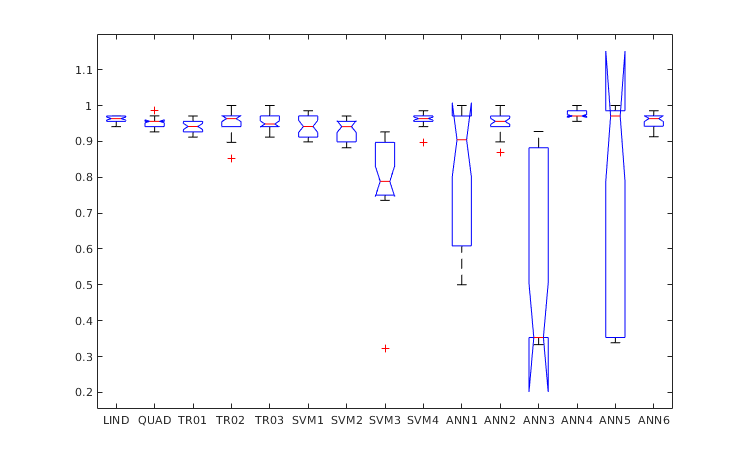
\includegraphics[width=0.6\textwidth]{img/box_cancer.bmp.png}
\caption{Cáncer}
\end{figure}

\begin{figure}[H]
\centering
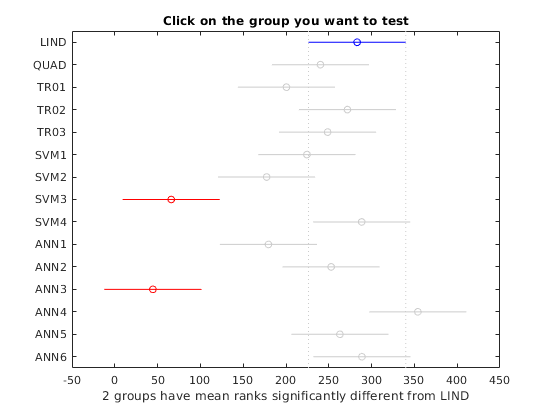
\includegraphics[width=0.6\textwidth]{img/ranks_cancer.bmp.png}
\caption{Cáncer}
\end{figure}

\begin{figure}[H]
\centering
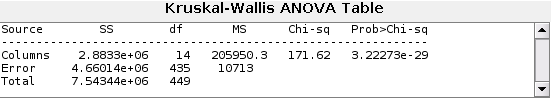
\includegraphics[width=0.6\textwidth]{img/anova_cancer.bmp.png}
\caption{Cáncer}
\end{figure}

\begin{figure}[H]
\centering
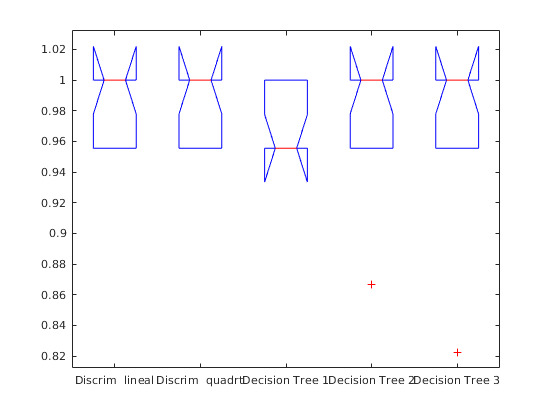
\includegraphics[width=0.6\textwidth]{img/box_iris.jpg}
\caption{Iris}
\end{figure}

\begin{figure}[H]
\centering
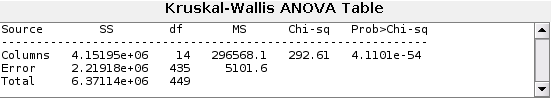
\includegraphics[width=0.6\textwidth]{img/anova_iris.bmp.png}
\caption{Iris}
\end{figure}

\begin{figure}[H]
\centering
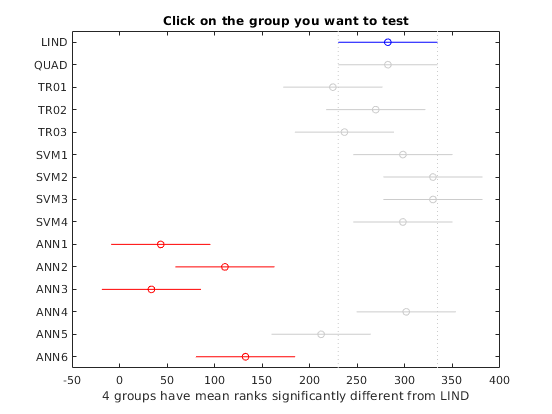
\includegraphics[width=0.6\textwidth]{img/ranks_iris.bmp.png}
\caption{Iris}
\end{figure}

\begin{figure}[H]
\centering
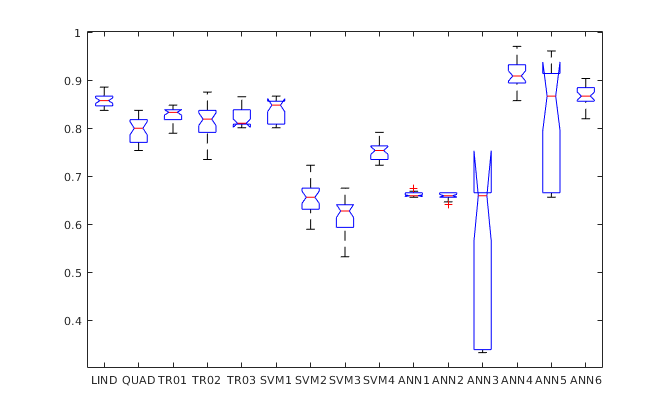
\includegraphics[width=0.6\textwidth]{img/box_biodeg.bmp.png}
\caption{Biodeg}
\end{figure}

\begin{figure}[H]
\centering
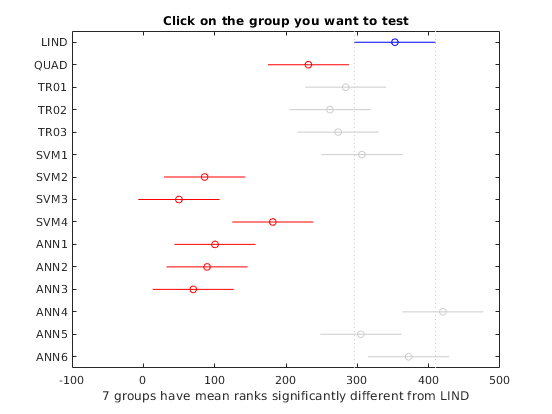
\includegraphics[width=0.6\textwidth]{img/ranks_biodeg.bmp.png}
\caption{Biodeg}
\end{figure}


\begin{figure}[H]
\centering
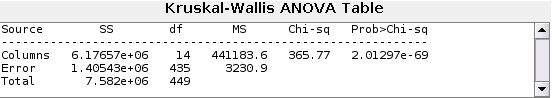
\includegraphics[width=0.6\textwidth]{img/anova_biodeg.bmp.png}
\caption{Biodeg}
\end{figure}

\section{Regresión}

\subsection{Resultados}
\begin{table}[H]
\centering
\begin{tabular}{@{}lll@{}}
\toprule
P-Value: 3.302e-94       & MSE( Train ) & MSE( Test ) \\ \midrule
SVM 1                    & 0.0032            & 0.0034           \\
SVM 2                    & 0.0036            & 0.0043           \\
SVM 3                    & 0.0035            & 0.0045           \\
SVM 4                    & 0.0055            & 0.0156           \\
ANN 1                    & 0.9977            & 0.9976           \\
ANN 2                    & 0.0087            & 0.0085           \\
ANN 3                    & 0.7307            & 0.7307           \\
ANN 4                    & 0.0061            & 0.0059           \\
ANN 5                    & 0.9535            & 0.9590           \\
ANN 6                    & 0.7237            & 0.7189           \\
ANN 7                    & 0.0019            & 0.0023           \\
ANN 8                    & 0.0004            & 0.0004           \\
ANN 9                    & 0.7311            & 0.7311           \\
ANN 10                   & 0.0067            & 0.0067           \\
ANN 11                   & 0.0006            & 0.0006           \\
ANN 12                   & 0.0012            & 0.7225           
\end{tabular}
\caption{Medidas globales de MSE en training y test(Henon)}
\label{tab:global_iris}
\end{table}


\begin{figure}[H]
\centering
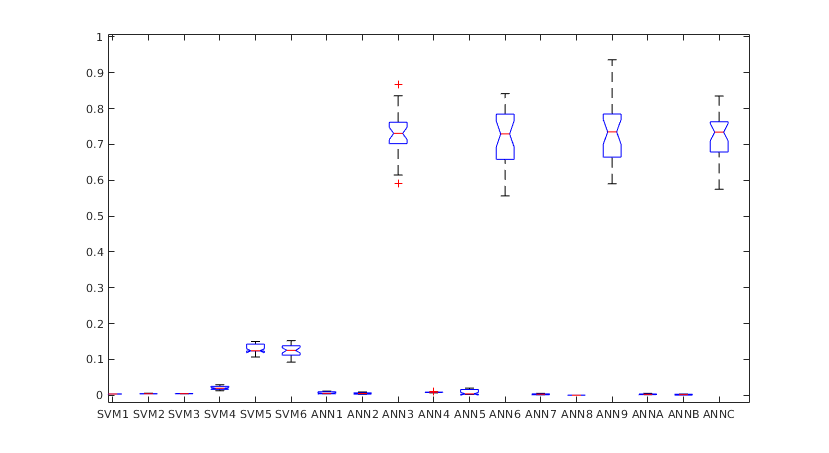
\includegraphics[width=0.6\textwidth]{img/box_henon.png}
\caption{Henon}
\end{figure}

\begin{figure}[H]
\centering
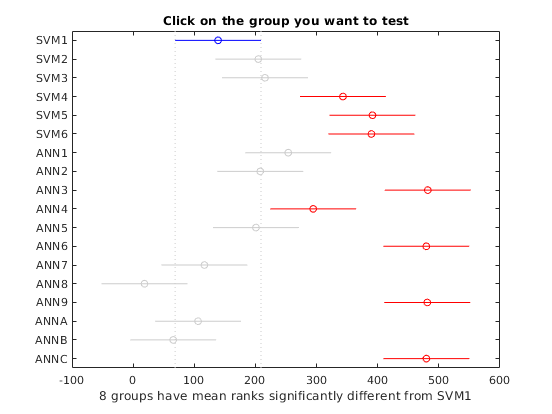
\includegraphics[width=0.6\textwidth]{img/ranks_henon.png}
\caption{Henon}
\end{figure}


\begin{figure}[H]
\centering
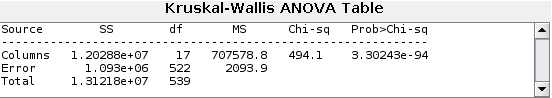
\includegraphics[width=0.6\textwidth]{img/anova_henon.png}
\caption{Henon}
\end{figure}

\newpage
\listoftables
\end{document}
